\section{Error Analysis}
\label{sec:errors}

\paragraph{Error types} Error types were given by three of the five annotators (A1, A4, A5; A2 and A3 gave labels only), so 21 of the 34 erroneous summaries have a final type (Fig.~\ref{fig:errortypes}b). \emph{Meaning} errors, in which correct names and numbers are put in a wrong relation, dominate: 14 of 21 final types, and 22 of the 32 typed error labels of the three annotators. Omissions that make a summary misleading follow (4 of 21); number, entity and added-information errors occur once each. This matches the automatic results: invented names and numbers are rare, so the precision metrics are at the ceiling, while the errors humans find are about relations. Thirty-three of the 34 erroneous summaries have perfect number and entity precision.

\paragraph{Relation errors that the automatic metrics pass} The three major errors below were labelled by the annotators; each has number and entity precision 1.0 (or no number), and each passes NLI-window.
\begin{itemize}
  \item \emph{Outcome reversal} (\cond{hinglish}, plain): a rain-shortened England--Pakistan ODI was abandoned with Pakistan on 46 for 1, but the summary says ``Pakistan ne 46 run mein ek wicket loss ke saath match jeeta'' (Pakistan won the match). NLI-window 0.80, NLI-chunk 0.28.
  \item \emph{Outcome reversal} (\cond{hinglish}, plain): an India--England Test was drawn with India on 391/9, but the summary says India ``England ko khatam kar diya'' (finished England off), although all scores, Root's 154 and Anderson's man-of-the-match award are copied correctly. NLI-window 0.75, NLI-chunk 0.28.
  \item \emph{Role reversal} (\cond{hi-rom}, factual): in the source, George Fernandes supports the vegetable vendors protesting against Reliance and condemns the police brutality against them; the summary says he \emph{supported} the police's brutal treatment of the vendors and attributes to him an assurance of full protection for Reliance Fresh that, in the source, was given by the Chief Minister. NLI-window 0.66, NLI-chunk 0.52.
\end{itemize}
The same pattern appears outside the labelled set. In a \cond{hi} plain summary, gemma3:4b writes that Boeing launched the Dreamliner in 1995; the source gives 1995 as the launch year of the Boeing 777. Both the number and the name occur in the source, so number and entity precision are 1.0, and NLI scores the summary 0.76 (chunk) and 0.82 (window).

\paragraph{Errors that the precision metrics do catch} The few non-relation errors are caught by the script-independent checks. A \cond{hi-rom} plain summary says ``char lakh'' (4 lakh) children run away from home every year, where the source has 4 lakh 40 thousand; the parsed values differ, so number precision drops to 0.86. A \cond{hi} plain summary of the India--England Test writes the full name ``James Anderson'' (in Devanagari) where the source names only ``Anderson''; the first name is correct world knowledge but not in the article, and entity precision drops to 0.83. Under our guidelines both count as errors, the second as added information.

\paragraph{Script-conversion errors} Romanization loses information that the model sometimes restores wrongly. In the \cond{hi-rom} version of an article on the Bihar floods, \dev{बाढ़} (\emph{baadh}, flood) is written \emph{barh}, because our romanization does not mark vowel length. Asked for a factual summary, gemma3:4b answered in Devanagari and back-transliterated \emph{barh} as \dev{बारह} (\emph{baarah}, twelve) four times, e.g.\ ``\dev{बारह पीड़ितों को भूखा नहीं रहने दिया जाएगा}'' (``the \emph{twelve} victims will not be left hungry'' instead of ``the flood victims''). The summary failed the script check, so it was excluded from the factuality metrics and counts only towards the wrong-language rate; had it been scored, the number parser would have read \dev{बारह} as an invented 12.

\paragraph{Metric failure cases} Exact number-word lists also cause false positives: the surname ``Das'' is read as 10 (\emph{das}). In the labelled set, however, the precision metrics never flagged a faithful summary; the main failure is the opposite one, missed relation errors. NLI fails in both directions: NLI-window passes 31 of 34 erroneous summaries, and NLI-chunk scores 13 of 26 faithful summaries below 0.5.

\begin{figure}[t]
  \centering
  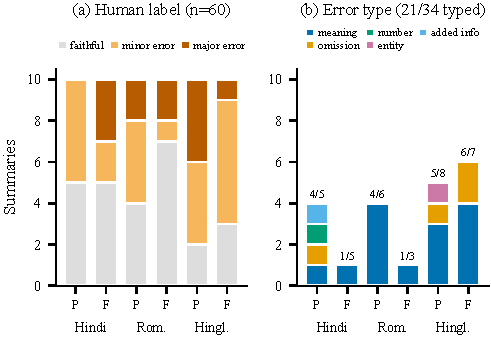
\includegraphics[width=\columnwidth]{fig_error_types}
  \caption{(a) Final human label of the 60 labelled gemma3:4b summaries (10 per condition and prompt; P = plain, F = factual). (b) Error type of the erroneous summaries that have one (typed / all errors above each bar); two of the five annotators gave no error types.}
  \label{fig:errortypes}
\end{figure}
